\documentclass{beamer}
\usepackage[latin1]{inputenc}

\usetheme{Madrid}
\usecolortheme{default}
\usepackage{amsmath}
\usepackage{amssymb,amsfonts,amsthm}
\usepackage{txfonts}
\usepackage{tkz-euclide}
\usepackage{listings}
\usepackage{adjustbox}
\usepackage{array}
\usepackage{tabularx}
\usepackage{gvv}
\usepackage{lmodern}
\usepackage{circuitikz}
\usepackage{tikz}
\usepackage{graphicx}
\usepackage{gensymb}
\usepackage{physics}

\setbeamertemplate{page number in head/foot}[totalframenumber]

\usepackage{tcolorbox}
\tcbuselibrary{minted,breakable,xparse,skins}



\definecolor{bg}{gray}{0.95}
\DeclareTCBListing{mintedbox}{O{}m!O{}}{%
  breakable=true,
  listing engine=minted,
  listing only,
  minted language=#2,
  minted style=default,
  minted options={%
    linenos,
    gobble=0,
    breaklines=true,
    breakafter=,,
    fontsize=\small,
    numbersep=8pt,
    #1},
  boxsep=0pt,
  left skip=0pt,
  right skip=0pt,
  left=25pt,
  right=0pt,
  top=3pt,
  bottom=3pt,
  arc=5pt,
  leftrule=0pt,
  rightrule=0pt,
  bottomrule=2pt,
  toprule=2pt,
  colback=bg,
  colframe=orange!70,
  enhanced,
  overlay={%
    \begin{tcbclipinterior}
    \fill[orange!20!white] (frame.south west) rectangle ([xshift=20pt]frame.north west);
    \end{tcbclipinterior}},
  #3,
}
\lstset{
    language=C,
    basicstyle=\ttfamily\small,
    keywordstyle=\color{blue},
    stringstyle=\color{orange},
    commentstyle=\color{green!60!black},
    numbers=left,
    numberstyle=\tiny\color{gray},
    breaklines=true,
    showstringspaces=false,
}
\title{2.10.54}
\date{5th september, 2025}
\author{Vishwambhar - EE25BTECH11025}

\begin{document}

\frame{\titlepage}
\begin{frame}{Question}
let $\vec{a, b,c}$ be unit vectors such that $\vec{a}+\vec{b}+\vec{c}=\vec{0}$. Which of the following are correct?\\
\begin{enumerate}
    \item $\vec{a}\times \vec{b}=\vec{b}\times \vec{c}=\vec{c}\times \vec{a}=\vec{0}$
    \item $\vec{a}\times \vec{b}=\vec{b}\times \vec{c}=\vec{c}\times \vec{a}\neq \vec{0}$
    \item $\vec{a}\times \vec{b}=\vec{b}\times \vec{c}=\vec{a}\times \vec{c}\neq \vec{0}$
    \item $\vec{a}\times \vec{b},\vec{b}\times \vec{c}, \vec{c}\times \vec{a}$ are mutually perpendicular.
\end{enumerate}
\end{frame}

\begin{frame}{Given}
Given:
\begin{align}
    \vec{a}+\vec{b}+\vec{c}=0\\
    \vec{c}= \myvec{\vec{a}&\vec{b}}\myvec{-1\\-1}\\
\end{align}
\end{frame}

\begin{frame}{Assuming 2D space}
This $\vec{c}$ lies in span of $\vec{a}, \vec{b}$.\\

Since $\vec{a}, \vec{b}, \vec{c}$ are all in 2D space, if all three are non-zero unit vectors satisfying this relation, they must be linearly dependent.\\

Therefore, the $2\times2$ matrix $\myvec{\vec{a}&\vec{b}}$ cannot be invertible.
\begin{align}
    \mdet{\myvec{\vec{a}&\vec{b}}}=0
\end{align}
\end{frame}

\begin{frame}{Singular matrix}
So the matrix is singular.

In 2D, norm is defined by the determinant:
\begin{align}
    ||\vec{a}\times\vec{b}||=\mdet{\myvec{\vec{a}&\vec{b}}}
\end{align}

So if $\mdet{\myvec{\vec{a}&\vec{b}}}=0$, then
\begin{align}
    \vec{a}\times\vec{b}=0
\end{align}
\end{frame}

\begin{frame}{conclusion}
Similarly, we can show the same for the vectors $\vec{a}$ and $\vec{b}$.

Thus, the correct option is (1):
\begin{align}
    \vec{a}\times \vec{b}=\vec{b}\times \vec{c}=\vec{c}\times \vec{a}=\vec{0}
\end{align}
\end{frame}


\begin{frame}[fragile]
    \frametitle{C Code}
    \begin{lstlisting}
#include <stdio.h>
#include <math.h>
typedef struct {
    double x, y, z;} 
    Vector;
Vector cross(Vector a, Vector b) {
    Vector result;
    result.x = a.y * b.z - a.z * b.y;
    result.y = a.z * b.x - a.x * b.z;
    result.z = a.x * b.y - a.y * b.x;
    return result;}
double dot(Vector a, Vector b) {
    return a.x * b.x + a.y * b.y + a.z * b.z;}
void check_conditions(Vector a, Vector b, Vector c, int *results) {
    Vector ab = cross(a, b);
    Vector bc = cross(b, c);
    Vector ca = cross(c, a);
    \end{lstlisting}
\end{frame}

\begin{frame}[fragile]
    \frametitle{C Code}
    \begin{lstlisting}
    // Option (a): all cross products = 0
    results[0] = (ab.x==0 && ab.y==0 && ab.z==0 &&
                  bc.x==0 && bc.y==0 && bc.z==0 &&
                  ca.x==0 && ca.y==0 && ca.z==0);
    // Option (b): all equal and nonzero
    results[1] = ((ab.x==bc.x && ab.y==bc.y && ab.z==bc.z) &&
                  (bc.x==ca.x && bc.y==ca.y && bc.z==ca.z) &&
                  !(ab.x==0 && ab.y==0 && ab.z==0));
    // Option (c): ab = bc = a*c != 0
    Vector ac = cross(a, c);
    results[2] = ((ab.x==bc.x && ab.y==bc.y && ab.z==bc.z) &&
                  (bc.x==ac.x && bc.y==ac.y && bc.z==ac.z) &&
                  !(ab.x==0 && ab.y==0 && ab.z==0));
    // Option (d): ab, bc, ca mutually perpendicular (dot = 0)
    results[3] = (fabs(dot(ab, bc)) < 1e-9 &&
                  fabs(dot(bc, ca)) < 1e-9 &&
                  fabs(dot(ca, ab)) < 1e-9);
}
    \end{lstlisting}
\end{frame}

\begin{frame}[fragile]
    \frametitle{Python Code 1}
    \begin{lstlisting}
import ctypes
from ctypes import c_double, c_int, POINTER
import math

# Load the shared object
lib = ctypes.CDLL("./libvectors.so")

# Define Vector struct
class Vector(ctypes.Structure):
    _fields_ = [("x", c_double), ("y", c_double), ("z", c_double)]

# Define function signature
lib.check_conditions.argtypes = [Vector, Vector, Vector, POINTER(c_int)]
lib.check_conditions.restype = None
    \end{lstlisting}
\end{frame}

\begin{frame}[fragile]
    \frametitle{Python Code 1}
    \begin{lstlisting}
# Example unit vectors (satisfying a+b+c=0)
a = Vector(1, 0, 0)
b = Vector(-0.5, math.sqrt(3)/2, 0)
c = Vector(-0.5, -math.sqrt(3)/2, 0)

# Results array
results = (c_int * 4)()
lib.check_conditions(a, b, c, results)

options = ['a', 'b', 'c', 'd']
for i, res in enumerate(results):
    print(f"Option {options[i]}: {'True' if res else 'False'}")
    \end{lstlisting}
\end{frame}

\begin{frame}[fragile]
    \frametitle{Python Code 2}
    \begin{lstlisting}
import sys
import numpy as np
import matplotlib.pyplot as plt

# Add local path for custom geometry functions
sys.path.insert(0, '/home/ganachari-vishwmabhar/Downloads/codes/CoordGeo')

# Import the given helper functions
from line.funcs import *
from triangle.funcs import *

# Define the vectors a, b, c (unit vectors with a+b+c=0)
a = np.array([1, 0])                         # Along x-axis
b = np.array([-0.5, np.sqrt(3)/2])           # 120° rotated
c = np.array([-0.5, -np.sqrt(3)/2])          # 240° rotated
    \end{lstlisting}
\end{frame}

\begin{frame}[fragile]
    \frametitle{Python Code 2}
    \begin{lstlisting}
# Plot the triangle formed by a, b, c
plt.figure()
xs = [a[0], b[0], c[0], a[0]]
ys = [a[1], b[1], c[1], a[1]]
plt.plot(xs, ys, 'k-', label='Triangle (a,b,c)')

# Mark the vectors from origin
O = np.array([0, 0])
plt.plot([O[0], a[0]], [O[1], a[1]], 'r-', label='a')
plt.plot([O[0], b[0]], [O[1], b[1]], 'g-', label='b')
plt.plot([O[0], c[0]], [O[1], c[1]], 'b-', label='c')
    \end{lstlisting}
\end{frame}

\begin{frame}[fragile]
    \frametitle{Python Code 2}
    \begin{lstlisting}
# Mark points
plt.scatter([a[0], b[0], c[0]], [a[1], b[1], c[1]], c=['r','g','b'])
plt.text(a[0], a[1], 'a', fontsize=12)
plt.text(b[0], b[1], 'b', fontsize=12)
plt.text(c[0], c[1], 'c', fontsize=12)

plt.axis('equal')
plt.grid(True)
plt.legend()
plt.title("Triangle of unit vectors (a+b+c=0)")
plt.savefig("../figs/plot.png")
plt.show()
    \end{lstlisting}
\end{frame}

\begin{frame}{Plot}
    \begin{figure}
        \centering
        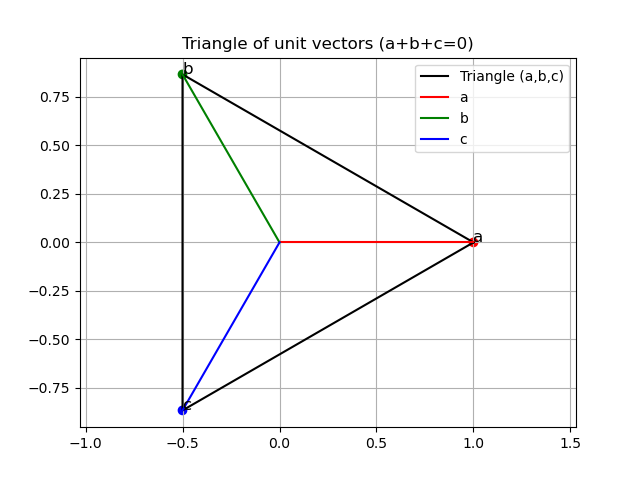
\includegraphics[width=0.5\columnwidth]{../figs/plot.png}
        \caption{Plot of vectors $\vec{a}, \vec{b}$ and $\vec{c}$}
        \label{fig:fig}
    \end{figure}
\end{frame}




\end{document}